\section{Dissertation Overview\label{sec:ch1:overview}}

This introduction has provided a discussion on the combined architecture, plant, and control design problems including how this problem type can be used in the dynamic system design process and some potential challenges.
Due to the diverse design domains considered in this dissertation, a variety of methodologies are presented to manage different elements in the design process.
Chapters \ref{ch:2}--\ref{ch:5} focus on the development of these methodologies while Chapters \ref{ch:6}--\ref{ch:8} present detailed engineering design case studies that utilize the concepts.
A focus in the initial chapters is on the generality of the proposed approaches.
The frameworks presented are developed with specific consideration of what types of problems will fit under the proposed framework.

\begin{itemize}
% new paragraph, architecture
\item Chapter~\ref{ch:2} focuses on the task of representing and generating candidate architectures.
The theory and algorithms developed in this chapter are applicable to architecture problems where the architecture is representable by a colored graph built from a catalog of components.
A complete listing of all potential architectures under specific assumptions can be generated with this approach.
A number of enhancements to the algorithms presented in this chapter are detailed in Appendix~\ref{app:A}.

% new paragraph, co-design
\item Chapter~\ref{ch:3} focuses on a methodology for handling the other two design domains: combined plant and control design or co-design.
The general co-design problem formulation and optimality conditions are explained for both the simultaneous and nested solution strategies.
Due to a number of challenges associated with the optimality conditions, practical solution  considerations are discussed with a focus on the motivating reasons for using direct transcription in co-design.

% new paragraph, scaling
\item Chapter~\ref{ch:4} concentrates on scaling in dynamic optimization (a general class of problems found in Chapter~\ref{ch:3}). 
The necessary theory for scaling dynamic optimization formulations is presented and a number of motivating examples are shown. 
Scaling can be used to help facilitate finding accurate, generalizable, and intuitive information. The unique structure of dynamic optimization suggests that scaling can be utilized in novel ways to provide better analysis and formulations more favorable for efficiently generating the solution. 
A simpler, scaled problem is used to understand the general trends found in the results of the case study in Chapter~\ref{ch:7}, along with minor roles in the other two case studies.

% new paragraph, direct transcription
\item Chapter~\ref{ch:5} presents the direct transcription method for finding approximate solutions to dynamic optimization problems.
The method discretizes (in time) the infinite-dimensional quantities and creates a mathematical program that can be solved.
This method is an enabling method that allows solutions to be obtained for general co-design problems in Chapter~\ref{ch:4}.
A bulk of the chapter is focused on solving a particular subclass: linear-quadratic dynamic optimization problems.
These problems can be approximated with quadratic programs and be efficiently constructed and solved.
Problems with this structure are particularly important when the three domains are considered because many control problems may need to be solved, and an inefficient method could hinder the ability to explore the solutions.
The algorithms, sparsity patterns, and example codes are in Appendix~\ref{app:C}.
The case studies in Chapter \ref{ch:7} and \ref{ch:8} utilize this theory and codes to solve the control subproblem.

% new paragraph, passive analog circuits
\item Chapter~\ref{ch:6} presents an enumeration-based synthesis methodology for passive analog circuits by generating and evaluating all appropriate circuits.
Two design problems are considered: frequency response matching and low-pass filter realizability.
The circuit graphs (architectures) are generated using the methods described in Chapter~\ref{ch:2}.
This problem contains both architecture and plant design decisions.

% new paragraph, strain-actuated solar arrays
\item Chapter~\ref{ch:7} focuses on the design of strain-actuated solar arrays for spacecraft precision pointing and jitter reduction.
This problem has a variety of challenging plant and control design variables.
The nested co-design strategy described in Chapter~\ref{ch:3} is utilized, and the control subproblem is solved with the methods in Chapter~\ref{ch:5}.
The primary example from Chapter~\ref{ch:4} provides a number of insights into the results found in this case study.

% new paragraph, vehicle suspensions
\item Chapter~\ref{ch:8} is a case study that combines all three design domains with the design of vehicle suspensions.
The work from Chapters~\ref{ch:2}--\ref{ch:5} all contribute in addressing this complex design problem.
This chapter also includes a discussion of a general class of architecture, plant, and control design problems that utilize linear physical elements.

% new paragraph, conclusion
\item Chapter~\ref{ch:9} concludes the dissertation with an overall summary of the key points and identifies future research directions.

\end{itemize}

\begin{figure}[hb]
\centering
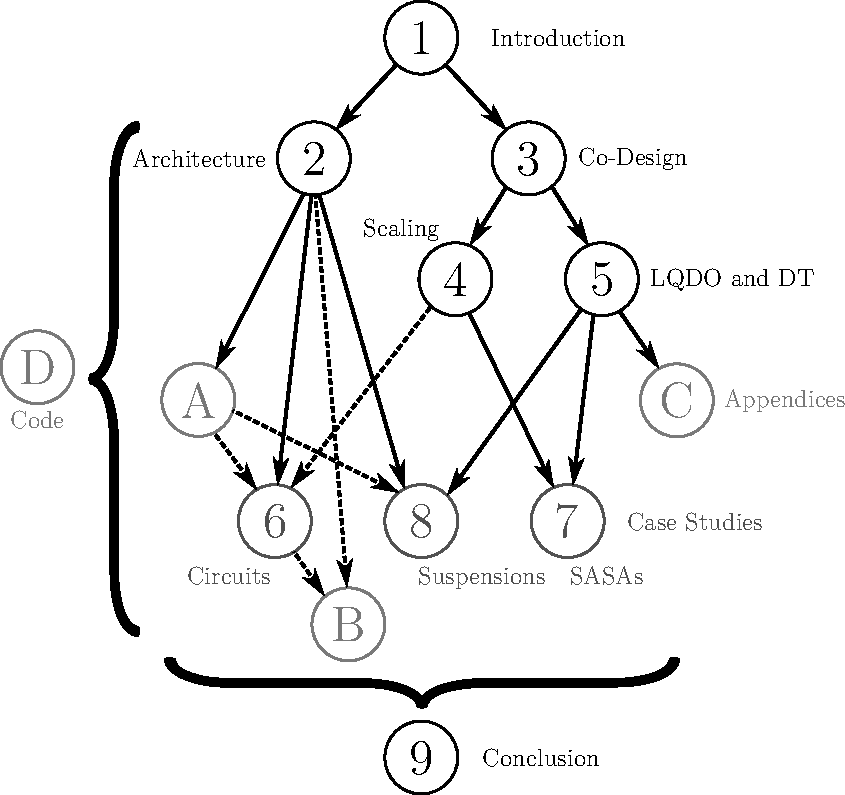
\includegraphics[width=0.65\textwidth]{../ch1/figures/outline2.pdf}
\caption[Dissertation content connections]{Dissertation content connections (dashed line indicates a narrower connection).\label{fig:ch1:outline}}
\end{figure}